\section{Chapter 5 - Problem (12)}
	A $3.8 \ kg$ block is pushed along a horizontal floor by a force $\vec{F}$ of magnitude $17 \ N$ at an angle $\theta = 29^{o}$ with the horizontal. The coefficient of kinetic friction between the block and the floor is $0.33$.

	\begin{figure}[H]
		\begin{center}
			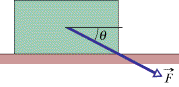
\includegraphics[scale=1]{hw6_problem12}
			\caption{Illustration of Problem 12}
			\label{fig:hw6_problem12}
		\end{center}
	\end{figure}

	\subsection{Question (a)}

		Calculate the magnitude of the friction force on the block from the floor:

		\textbf{R:} \newline

		\begin{figure}[H]
			\begin{center}
				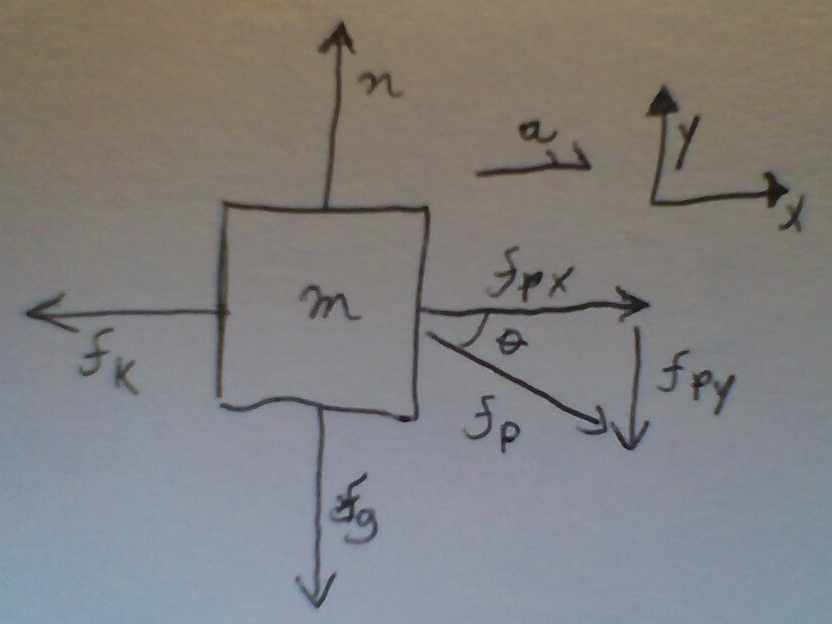
\includegraphics[scale=0.3]{hw6_problemc_fbd}
				\caption{Free-Body Diagram (Problem 12)}
				\label{fig:hw6_problemc_fbd}
			\end{center}
		\end{figure}

		\begin{align}
			f_{k} = \ &\mu_{k}n& \notag
		\end{align}

		Newton's $2^{nd}$ Law to discover $n$:

		\begin{align}
			\sum F_{y} = \ &ma_{y}& \notag \\
			n - mg - f_{p_{y}} = \ &m(0)& \notag \\
			n = \ &mg + (f_{p} \sin 29^{o})& \notag \\
			= \ &\left[(3.8 \ kg)\left(9.80 \ m/s^{2}\right)\right] + \left[(17 \ N)(0.48481)\right]& \notag \\
			= \ &(37.24 \ N) + (8.2418 \ N)& \notag \\
			= \ &45.482 \ N& \notag
		\end{align}

		\begin{align}
			f_{k} = \ &(0.33)(45.482 \ N)& \notag \\
			= \ &15.009 \ N&
		\end{align}

	\subsection{Question (b)}

		Calculate the magnitude of the block's acceleration:

		\textbf{R:} \newline

		Newton's $2^{nd}$ Law:
		\begin{align}
			\sum F_{x} = \ &ma_{x}& \notag \\
			f_{p_{x}} - f_{k} = \ &ma_{x}& \notag \\
			a = \ &\frac{\left[(17 \ N) \cos 29^{o}\right]  - (15.009 \ N)}{3.8 \ kg}& \notag \\
			= \ &\frac{(14.869 \ N)  - (15.009 \ N)}{3.8 \ kg}& \notag \\
			= \ &\frac{-0.14 \ N}{3.8 \ kg}& \notag \\
			= \ &-0.037 \ m/s^{2}&
		\end{align}
